\chapter{Methods and Implementations}

\section{Dataset Collection}
In order to evaluate and test the various schemes discussed in this paper, we conducted controlled experiments to capture and label head position and orientation data along the spiral path. Two primary data sources were utilized: sensor measurements, including data from a 9 Degrees of Freedom (DOF) sensor and a barometric pressure sensor, and network signals captured from routers at the target environment.

\subsection{Ground Truth Data}
To measure accurate ground truth data, the RTAB-MAP application (Real-Time Appearance-Based Mapping) was used. RTAB-MAP is a Simultaneous Localization and Mapping (SLAM) framework that uses RGB-D, stereo, and LiDAR technologies, as well as graph-based incremental appearance-based loop closure detection. In general, SLAM involves emitting laser pulses, analyzing their return times, and generating 3D point clouds that represent the environment. The data can then be used to determine a subject's position and orientation. For more details, one can refer to the RTAB-MAP website \cite{rtabmap} and Wevolver's LiDAR SLAM article. \cite{malik_2023_lidar}
\par
The process of collecting ground truth data involved initializing RTAB-MAP on an iPhone, starting a new data recording session, and walking along the designated spiral path. To make sure that the recorded data was as accurate as possible, the phone's camera was kept unobstructed throughout the recording. RTAB-MAP's output, which is sufficiently accurate for this project, was used as the benchmark ground truth data.

\subsection{Sensor Data}
During the collection of ground truth data, the Arduino setup was activated, and the subject walked along the spiral path to collect raw sensor data. By integrating and processing the collected raw measurements, the subject's orientation and position were estimated. The Wi-Fi data was collected using a 2nd Arduino microcontroller, which exclusively scanned for RSSI values. The data was retrieved by the main Arduino module via a UART connection.

\subsection{Measurement Apparatus}
To simulate real-world conditions, measurements were conducted with the sensors attached to headphones, replicating their intended final placement. A custom measurement device (\cref{measurementapparatus}) was used to ensure accurate data collection. This device was then attached to the headphones as can be seen on \cref{measurementapparatus}. With this approach, the collected data accurately reflected the end-use scenario, making it reliable for realistic position and orientation estimation.

\begin{figure}[h] 
	\centering 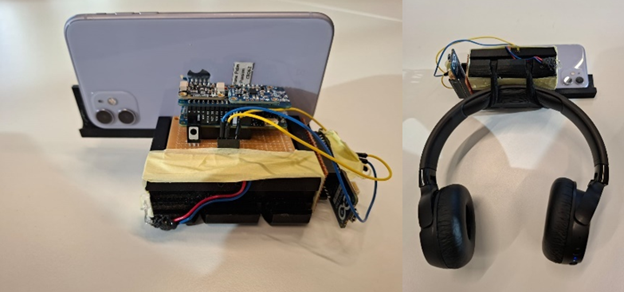
\includegraphics[height=4cm]{./images/apparatus.png}
	\caption{The 3D printed measurement apparatus.}
	\label{measurementapparatus}
\end{figure}

\subsection{Data Collection Process}
After setting up the measurement device, the data was collected. The data collection was done on the spiral of the GroupT campus in Leuven, Belgium. For each data recording session, the person wearing the measurement device must start and end the session at the same point, more precisely at the beginning of the spiral. In addition, the person stops at the same point, more precisely at the top of the spiral, before heading back to the starting position. Every measurement session lasts 10 minutes, but extending the duration can improve accuracy.
\par
Two types of measurements were taken. The first one represents an ideal sequence where the subject walks along the middle of the spiral in a straight line, with no interference, steady pace, and limited head rotation. The second type of measurement involves the person who is collecting data to walk along the spiral while applying more natural and random movements, such as moving up and down multiple times, moving the head in random orientations, moving away from the center of the spiral's path, etc. In total, 1 hour and 50 minutes of data was collected.

\section{Dataset Preprocessing}
After collecting our dataset, it had to be preprocessed in multiple ways before it was usable with our systems and evaluations. First of all, the data is sent from the Arduino to the desktop python environment where it's processed further.

\subsection{Synchronization}
Since the Arduino data and the ground truth data are running on two separate independently clocked systems, a synchronization step is required first. To do this, a computer vision-based synchronization mechanism was implemented. 
\par
As previously mentioned, both the raw data collection setup and the iPhone were mounted on a single measurement apparatus. An LED, connected to the Arduino, was positioned in the iPhone camera's field of view. Such LED lights up when the sensors connected to the Arduino are collecting data, serving as a synchronization marker. Using the OpenCV library, the irrelevant SLAM data that was recorded when the LED was off was filtered out. In addition, the sampling frequency of the raw data was much higher than the sampling frequency of the ground truth data, meaning that at the end of each recording session there were less ground truth samples than raw ones. Because of this, linear interpolation was used to match the oversampled raw data to the closest SLAM data points.

\subsection{Alignment and Normalization}
Due to the inconsistent starting orientations and initial conditions, the ground truth data isn't always aligned to the same origin. In order to ensure our evaluation was valid, we implemented a data preprocessing step that ensures the entire dataset is aligned in 3d space. The implementation first ensures all the spirals are centered about the same point, and then aligns the starting points of the aligned spirals.

\begin{figure}[h] 
	\centering 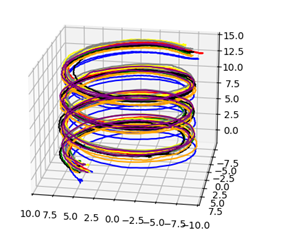
\includegraphics[height=5cm]{./images/aligned_data.png}
	\caption{The aligned spiral data.}
\end{figure}

After the alignment step, the sensor data is normalized so that the initial measurements are the "baseline values". Orientation data has the initial measurement subtracted from all measurements, resulting in it starting at the orientation origin. The ground truth orientation is similarly processed, however in quaternion space. Finally, the pressure data is preprocessed to remove outlier values due to sensor errors.

\section{Dataset Storage}
After synchronization, the data is stored so that it can be further processed. More precisely, the data was stored in HDF5 format (Hierarchical Data Format version 5). More precisely, the data for each full measurement session is stored in one HDF5 file which consists of the ground truth data, the raw data, and the Wi-Fi data. HDF5 format was used for data storage due to its multiple advantages such as its ability to store large datasets in structured hierarchy. The format is presented below.  \cite{hierarchical}
\par
\begin{table}[h!]
\centering
\renewcommand{\arraystretch}{1.1} % Reduce row height
\setlength{\tabcolsep}{8pt} % Reduce column spacing
\begin{tabular}{|l|l|}
\hline
\textbf{Group / Category} & \textbf{Subcategories} \\ \hline
\multirow{3}{*}{GT\_DATA}  & ORIENTATION            \\ \cline{2-2}
                           & POSITION               \\ \cline{2-2}
                           & TIMESTAMP              \\ \hline
\multirow{6}{*}{RAWDATA}   & 9DOF                   \\ \cline{2-2}
                           & BMP                    \\ \cline{2-2}
                           & BNO                    \\ \cline{2-2}
                           & PRESSURE               \\ \cline{2-2}
                           & RPY                    \\ \cline{2-2}
                           & TIMESTAMP              \\ \hline
\multirow{4}{*}{WIFIDATA}  & BSSIDS                 \\ \cline{2-2}
                           & COUNTS                 \\ \cline{2-2}
                           & RSSIS                  \\ \cline{2-2}
                           & TIMESTAMP              \\ \hline
\end{tabular}
\caption{Structure of an HDF5 file}
\label{tab:hdf5_structure}
\end{table}

\section{Synthetic Data Generation}
An additional synthetic data pipeline was implemented in order to achieve 3 main goals: providing an alternative to tedious data collection procedures, allowing for quick prototyping of algorithms and schemes before the full dataset was collected, and ensure behavioral integrity and reliability of implemented schemes before real evaluations. Since the required synthetic data generation was not meant to replace the actual dataset, we opted for a simple mathematical model for the sensor outputs, followed by sampled white gaussian noise.
\par
The implemented pipeline is able to generate artificial sensor readings for any given "ground truth" trajectory, whether that trajectory is actual collected data, or synthetically generated positions. Using a simple discrete derivative formula, the velocities and accelerations were calculated from the input positions, and the rotations were calculated as the tangents to the synthetic spiral. Following that, the pressure value is calculated using the altitude-pressure formula \cite{barometric} and white gaussian noise is added to the measurements.
\par
Furthermore, artificial Wi-Fi RSSI data was added to the synthetic data pipeline, using defined BSSIDs in certain positions, and the distance-RSSI formula. \cite{shang_2014_a} Finally, all this data is stored similarly to the actual dataset, in an identically formatted HDF5 sequence, to allow for interchangeability between the real and synthetic sequences.



\section{Position Estimation}
\subsection{Naive Double Integration Dead Reckoning}
The simplest and most well-known approach to positioning using IMU data is naive double integration dead reckoning (NDI) \cite{yan_2019_ronin}, where the acceleration components are discretely integrated into velocities, which are then in turn integrated into positions. The issue with this approach is that due to the double integration, sensor offsets, and noise can easily snowball due to the double integration procedure and as such the predictions drift very quickly. \cite{yan_2019_ronin}. In experiments with NDI, the algorithm's predictions went out of control very quickly. Due to these issues, NDI is not a solution for the indoor positioning problem.

\begin{figure}[h] 
	\centering 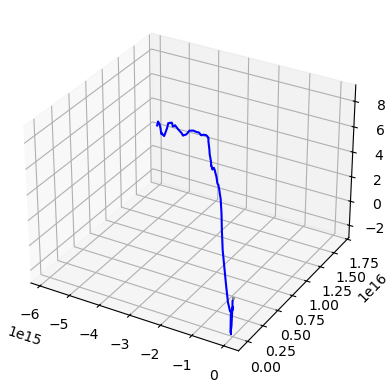
\includegraphics[height=5cm]{./images/ndi.png}
	\caption{The massive drift issues apparent in NDI.}
\end{figure}

\subsection{Pressure and Environment Model Based Positioning}
The next positioning method we explored was using the BMP390 pressure sensor's pressure values, along with our environment model for the spiral environment.
\subsubsection{Pressure Based Altitude Estimation}
Using the following formula, we determined the height values using the pressure data received.
$$P\left(z\right)=P_0e^{-\alpha z}$$

Using the derived pressure values, we calculate a 3D position in the target environment using a direct mapping from altitude values to 3D positions built on information about the target environment. Using information from both our ground truth data in our collected dataset, and ground plan data of the target environment. The mathematical model implements a mathematically ideal spiral, with its parameters tuned to best fit the ground truth data and the floor plan data. After visual tuning and comparing values with the ground plans, the parameters finally used are shown below, along with a diagram showing the ground truth data next to the model data.

\begin{figure}[h] 
	\centering 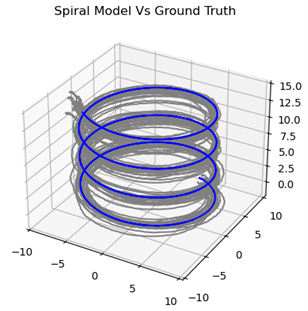
\includegraphics[height=5cm]{./images/spiralmodel.png}
	\caption{A visualization of the derived spiral model (blue) and the ground truth data (gray).}
\end{figure}

\begin{table}[h!]
\centering
\renewcommand{\arraystretch}{0.9} % Reduce row height
\setlength{\tabcolsep}{6pt}       % Reduce column spacing
\begin{tabular}{|l|c|}
\hline
\textbf{Parameter}       & \textbf{Value (m)} \\ \hline
\texttt{spiral\_pitch}   & 4.2               \\ \hline
\texttt{spiral\_radius}  & 8.0               \\ \hline
\texttt{path\_width}     & 2.4               \\ \hline
\end{tabular}
\vspace{-0.5em}
\caption{Parameters of the spiral model.}
\label{tab:spiral_params}
\end{table}
\par

The spiral mathematical model was furthermore developed with functionality to align them with ground truth data spirals, to allow for more accurate inference. This is done via calculating the maximum bounds along the x and y axes of the spiral, and then using the resulting centroid as the center of the spiral. Furthermore, the spiral model is capable of deriving a 3D position using a Z value using the formulas below.
$$\theta=2\pi\frac{z}{p}$$
$$x=x_0+r\cdot cos\left(\theta+\varphi\right)$$
$$y=y_0-\ r\cdot sin\left(\theta+\varphi\right)$$ 

Where theta is the angle on the circular top-down projection of the spiral, x, y, z are the 3D positions of the output point (and z is the input height), phi is the phase shift of the spiral calculated at alignment, r is the radius of the spiral, p is the pitch of the spiral, and $x_0$ and $y_0$ are the center x and y position of the spiral's top-down projection.
Additionally, the model is capable of calculating the closest point on the spiral model to an arbitrary input point. The distance between an arbitrary point and a point on the spiral was derived mathematically in cylindrical space, using $r_{sp}$, $h_{sp}$, and $\theta_{sp}$ as the position of the closest point on the spiral to the arbitrary point $r_{pt}$, $h_{pt}$, and $\theta_{pt}$. Then an optimization problem was solved by solving $d^2\prime$ = 0. The formulas for this problem are shown below

$$d^2=r_{sp}^2+r_{pt}^2-2r_{sp}r_{pt}cos\left(\theta_{sp}-\theta_{pt}\right)+\left(h_{sp}-h_{pt}\right)^2$$
$$\theta_{sp}=2\pi\frac{h_{sp}}{p}$$
$$\frac{{d(d}^2)}{d(h_{sp})}=\ \frac{4\pi r_{sp}r_{pt}}{p}sin(\frac{2\pi h_{sp}}{p}-\theta_{sp})+2h_{sp}-2h_{pt}$$

After the formula above was derived, finding a solution analytically was difficult, and solvers were unable to compute a solution due to the periodicity of the sine section of the formula. As a result, we opted for a polynomial half period approximation of a sine wave  and used a symbolic solver to derive the candidate solutions for the optimal point. There are 3 candidate solutions, we choose the solution that produces the lowest distance and return the point at the resulting $h_{sp}$. 

$$sin\ x\ \approx\ \frac{16x(\pi-x)}{5\pi^2-4x(\pi-x)}$$

\subsection{Wi-Fi Based Positioning}
Given the ubiquitous nature of Wi-Fi networks, using Wi-Fi data for positioning is a very attractive approach. Additionally, the target environment, being a university campus, was filled with constant position Wi-Fi networks, which could be used as anchors for a fingerprinting system. To this end, we implemented a random forest regressor model and trained it over our dataset in order to predict 3D positions using the detected BSSID to RSSI data measured from the Arduino's Wi-Fi module. \cite{pedregosa_2011_scikitlearn}
\par

The model's input format is a vector of RSSI values, with each position being associated with a unique Wi-Fi BSSID found in the training set. During inference, any BSSIDs not found in the dataset are disregarded, and any BSSIDs found have their associated RSSI values placed at the corresponding position in the input vector. Any undetected BSSIDs in the input vector are set to a value of -100dB.
\par

A grid search was conducted over the number of estimators and the maximum depth, and the following model hyperparameters were determined to perform best for our task. The results of the grid search are shown along with the model's hyperparameters in \cref{tab:model_hyperparameters}.
\par
\begin{table}[h!]
\centering
\renewcommand{\arraystretch}{1.1} % Adjust row height
\setlength{\tabcolsep}{8pt}       % Adjust column spacing
\begin{tabular}{|l|l|}
\hline
\textbf{Parameter}                 & \textbf{Value}             \\ \hline
\texttt{bootstrap}                 & True                       \\ \hline
\texttt{ccp\_alpha}                & 0.0                        \\ \hline
\texttt{criterion}                 & 'squared\_error'           \\ \hline
\texttt{max\_depth}                & 28                         \\ \hline
\texttt{max\_features}             & 1.0                        \\ \hline
\texttt{max\_leaf\_nodes}          & None                       \\ \hline
\texttt{max\_samples}              & None                       \\ \hline
\texttt{min\_impurity\_decrease}   & 0.0                        \\ \hline
\texttt{min\_samples\_leaf}        & 1                          \\ \hline
\texttt{min\_samples\_split}       & 2                          \\ \hline
\texttt{min\_weight\_fraction\_leaf} & 0.0                      \\ \hline
\texttt{monotonic\_cst}            & None                       \\ \hline
\texttt{n\_estimators}             & 525                        \\ \hline
\texttt{n\_jobs}                   & None                       \\ \hline
\texttt{oob\_score}                & False                      \\ \hline
\texttt{random\_state}             & None                       \\ \hline
\texttt{verbose}                   & 0                          \\ \hline
\texttt{warm\_start}               & False                      \\ \hline
\end{tabular}
\caption{Model Hyperparameters.}
\label{tab:model_hyperparameters}
\end{table}
\par

\subsection{Kalman Filtering Schemes}
Using a combination of the IMU's accelerometer data with the NDI method, and the BMP390's pressure data and the derived altitudes, we implemented our first Kalman filtering scheme, which fuses the data from these two sources to attempt to find a more accurate output. The Kalman filter was implemented with a state vector containing the positions and velocities along the x, y, and z axes. A mathematical formulation of the filter is shown below. These filters were then tuned by a scalar parameter scaling these matrices.
\par
\[
H_{\text{PRESSURE}} =
\begin{bmatrix}
1.0 & 0.0 & 0.0 & 0.0 & 0.0 & 0.0 \\
0.0 & 1.0 & 0.0 & 0.0 & 0.0 & 0.0 \\
0.0 & 0.0 & 1.0 & 0.0 & 0.0 & 0.0 \\
\end{bmatrix}
\]
\begin{center}
\textbf{Matrix 1:} Measurement matrix for pressure state variables.
\end{center}


\[
H_{\text{WIFI}} =
\begin{bmatrix}
1.0 & 0.0 & 0.0 & 0.0 & 0.0 & 0.0 \\
0.0 & 1.0 & 0.0 & 0.0 & 0.0 & 0.0 \\
0.0 & 0.0 & 1.0 & 0.0 & 0.0 & 0.0 \\
\end{bmatrix}
\]
\begin{center}
\textbf{Matrix 2:} Measurement matrix for WiFi state variables.
\end{center}


\[
A =
\begin{bmatrix}
1.0 & 0.0 & 0.0 & \Delta t & 0.0 & 0.0 \\
0.0 & 1.0 & 0.0 & 0.0 & \Delta t & 0.0 \\
0.0 & 0.0 & 1.0 & 0.0 & 0.0 & \Delta t \\
0.0 & 0.0 & 0.0 & 1.0 & 0.0 & 0.0 \\
0.0 & 0.0 & 0.0 & 0.0 & 1.0 & 0.0 \\
0.0 & 0.0 & 0.0 & 0.0 & 0.0 & 1.0 \\
\end{bmatrix}
\]
\begin{center}
\textbf{Matrix 3:} State transition matrix.
\end{center}

\[
B =
\begin{bmatrix}
0.5\Delta t^2 & 0.0 & 0.0 \\
0.0 & 0.5\Delta t^2 & 0.0 \\
0.0 & 0.0 & 0.5\Delta t^2 \\
\Delta t & 0.0 & 0.0 \\
0.0 & \Delta t & 0.0 \\
0.0 & 0.0 & \Delta t \\
\end{bmatrix}
\]
\begin{center}
\textbf{Matrix 4:} Control transition matrix.
\end{center}

\par
The filter's covariance and noise matrices were tuned by hand and evaluated over dataset sequences in order to choose the best performing values.
\par
Another architecture we experimented with was incorporating the Wi-Fi positioning data as well into the Kalman filtering scheme. This Kalman filter used the same state vector and transition matrix, however, the filter was updated using both the pressure-altitude based positions and the Wi-Fi positioning data.

\section{Orientation Estimation}
The second step of the head-tracking system was implementing an attitude estimation system. Our implemented attitude system uses the BNO055 IMU's orientation estimation system, with some further postprocessing. The data is retrieved as roll, pitch, yaw Euler angles in degrees, and are baselined on an initial assumption of the user starting approximately at the orientation origin. \cite{bno055}

\section{Real-Time Communication}
The final step of the head-tracking system was ensuring the system can run in real-time and not just on the collected dataset. Given that our signal processing schemes were implemented to run in a python desktop environment and were incapable of running on the microcontroller, we had to set up real-time network communication between the system and the python environment. We implemented two interchangeable communication layers; one built on TCP, and one built on UDP. The UDP system is preferred and was used for our data collection and real-time testing, since the system is more efficient and robust to packet drops. The system relies on two internal data structures used to represent the sensor data and the Wi-Fi data respectively.
\par

 \noindent\small
\begin{table}[h!]
\centering
\resizebox{\linewidth}{!}{ % Resize table to fit column width
\begin{tabular}{|l|l|l|l|}
\hline
\textbf{Type}            & \textbf{Name}                     & \textbf{Size (bytes)}   & \textbf{Notes}              \\ \hline
\texttt{unsigned long}   & \texttt{microsT}                  & 4                      & 4 bytes padding             \\ \hline
\texttt{double}          & \texttt{linaccelx, linaccely, linaccelz} & $8 \times 3 = 24$ & Linear acceleration         \\ \hline
\texttt{double}          & \texttt{gyrox, gyroy, gyroz}      & $8 \times 3 = 24$      & Gyroscope values            \\ \hline
\texttt{double}          & \texttt{magnx, magny, magnz}      & $8 \times 3 = 24$      & Magnetometer values         \\ \hline
\texttt{double}          & \texttt{roll, pitch, yaw}         & $8 \times 3 = 24$      & Orientation values          \\ \hline
\texttt{int8\_t}         & \texttt{tempnbo}                  & 1                      & 7 bytes padding             \\ \hline
\texttt{double}          & \texttt{tempbmp}                  & 8                      & Temperature                 \\ \hline
\texttt{double}          & \texttt{pressure}                 & 8                      & Pressure                    \\ \hline
\end{tabular}
}
\caption{Structure of \texttt{DataEntry} (Size: 128 bytes).}
\label{tab:dataentry}
\end{table}

\noindent\small
\begin{table}[h!]
\centering
\resizebox{\linewidth}{!}{ % Resize table to fit column width
\begin{tabular}{|l|l|l|l|}
\hline
\textbf{Type}            & \textbf{Name}               & \textbf{Size (bytes)}   & \textbf{Notes}              \\ \hline
\texttt{unsigned long}   & \texttt{microsT}            & 4                      & -                           \\ \hline
\texttt{int8\_t}         & \texttt{rssiCnt}            & 1                      & 1 byte padding              \\ \hline
\texttt{byte}            & \texttt{BSSIDs[25][6]}      & $25 \times 6 = 150$    & 1 byte padding              \\ \hline
\texttt{int32\_t}        & \texttt{RSSIs[25]}          & $25 \times 4 = 100$    & -                           \\ \hline
\end{tabular}
}
\caption{Structure of \texttt{RssiDataEntry} (Size: 256 bytes).}
\label{tab:rssidatadataentry}
\end{table}

\par

\section{Visualization}

To visualize data in real-time, we initially used matplotlib's Animation module for simple animations to validate our solution. However, due to its limitations, we switched to Blender, a free 3D graphics software known for realistic 3D rendering, camera, lighting, and material options, and Python scripting capabilities. 
We first animated the ground truth and unfiltered data in Blender, using the data from h5 files. Once confirmed to be working as expected, we modeled the real-time data from our implementation.
\par
Blender includes its own Python environment, requiring the installation of necessary Python libraries within Blender's Python. Since the filtering script and Blender visualization ran in separate Python environments, we established communication between them using TCP sockets. The main Python script acted as a server, sending orientation and position data to the Blender script, which acted as a client, receiving the data.
\par
We modeled the spiral, floor, and walls in 3D, adding lighting and camera tracking. In the final Blender file, a face is visible in the main frame, adjusting the camara to follow along the spiral as a person ascends.
Blender on our PCs could render at a maximum of 25 frames per second (fps), while our solution sampled at 100Hz. To synchronize the visualization with real-time position and orientation, we sent only one sample of position and orientation data out of every four samples to the Blender script.
\cref{viz} displays the final Blender animation. On the right is the camera view, focusing on the monkey face at the center. On the left is a overview visualization of all the objects that were modeled.

\begin{figure}[h] 
	\centering 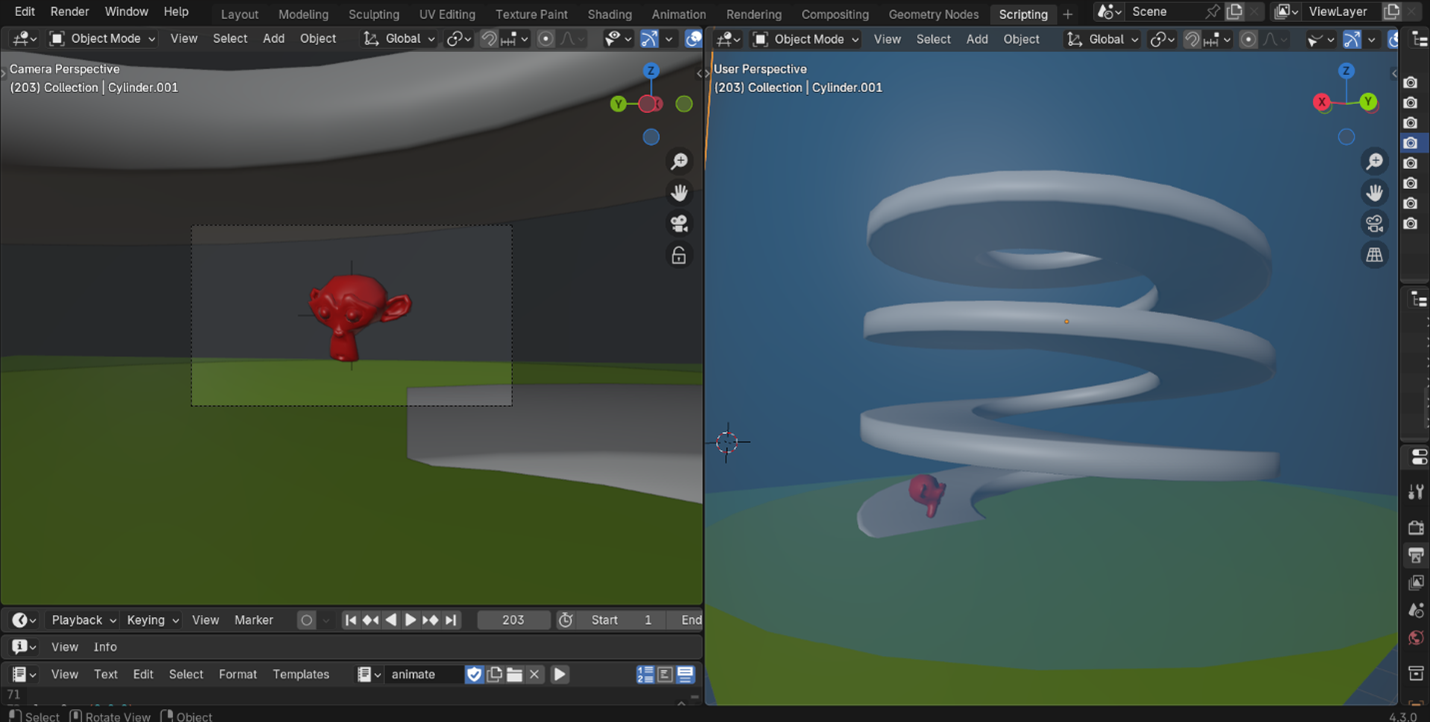
\includegraphics[height=4cm]{./images/visualization.png}
	\caption{A preview of the implemented visualizer.}
	\label{viz}
\end{figure}

